\documentclass[a4paper,12pt]{report}
\usepackage[utf8]{inputenc}
\usepackage[french]{babel}
\usepackage[top=3cm, bottom=3cm, left=2cm, right=2cm]{geometry}
\usepackage[T1]{fontenc}
\usepackage{graphicx}
\usepackage{hyperref}
\usepackage{tikz}
\usepackage{color}
\usepackage{colortbl}
\usepackage{multirow}
\usepackage{listings}
%%%%%%%%%%%%%%%%%%%%%%%%%%%%%%%%%%%%%%%%%%%%%%%%%%%%%%%%%%%%%%%%%%%%%%%
\begin{document}
%%%%%%%%%%%%%%%%%%%%%%%%%%%%%%%%%%%%%%%%%%%%%%%%%%%%%%%%%%%%%%%%%%%%%%%

\begin{titlepage}
    \begin{center}
        \begin{tikzpicture}[remember picture,overlay]
            \node[xshift=5.5cm, yshift=-3.6cm] at (current page.north west) {
\includegraphics[scale=0.5]{logo-insa.jpg}};
            \node[xshift=15.5cm, yshift=-3.6cm] at (current page.north west) {
\includegraphics[scale=0.18]{logo-asi.jpg}};
        \end{tikzpicture}
        \newline{} \newline{} \newline{} \newline{}
        \huge{\bsc{Document \& Web Sémantique}} \\
        \rule{\linewidth}{1.5pt}
        \huge{\textbf{Reconnaissance de Formes}}
        \rule{\linewidth}{1.5pt} \newline{} \newline{}
    \end{center}
    \textit{Auteurs : \hfill Evaluateur :} \\ Julien \bsc{Baron} \hfill Clément \bsc{Chatelain} \\ 
                                                Grégoire \bsc{Gutzwiller} \\ \\
    \large{\underline{Cadre du projet : }} \\ \\
    \normalsize{L'objectif du projet est d'appréhender les différentes
        étapes d'un système de reconnaissance de formes à travers le
        développement d'une chaîne de reconnaissance de chiffres 
        manuscrits sous MATLAB.} \\ \\
    \begin{center}
        \textit{Date :} \\ 06 Mars 2015
    \end{center}
\end{titlepage}

%%%%%%%%%%%%%%%%%%%%%%%%%%%%%%%%%%%%%%%%%%%%%%%%%%%%%%%%%%%%%%%%%%%%%%%
\tableofcontents
%%%%%%%%%%%%%%%%%%%%%%%%%%%%%%%%%%%%%%%%%%%%%%%%%%%%%%%%%%%%%%%%%%%%%%%

\chapter*{Introduction}
\addcontentsline{toc}{chapter}{Introduction}
Au sein de l'EC Document, nous avons été amenés à travailler
avec M. Chatelain sur les méthodes de reconnaissance d'écriture.
Ces méthodes permettent, entre autres, de reconnaître de 
l'écriture humaine afin de la transformer un caractère numérique
lisible par un ordinateur. \\
L'objectif de ce projet est donc de mettre en pratique ce que
nous avons vu en cours sur la reconnaissance de formes et de nous
livrer à un exercice de recherche sur les meilleures façons de 
reconnaître des chiffres écrits à la main. \\
Nous allons donc avoir besoin de créer un programme MATLAB
permettant, à partir d'une base d'apprentissage, de déterminer les
nombres présents dans une base de test. Vous trouverez donc dans
ce rapport toute notre démarche pour atteindre un résultat le plus
proche possible de la perfection. 

\chapter{Les données}
Ce que nous appelons données consiste en fait en l'ensemble de la
base de test, et de la base d'apprentissage. Elles nous sont 
données sous la forme d'images que voici.

\begin{figure}[!h]
\centering
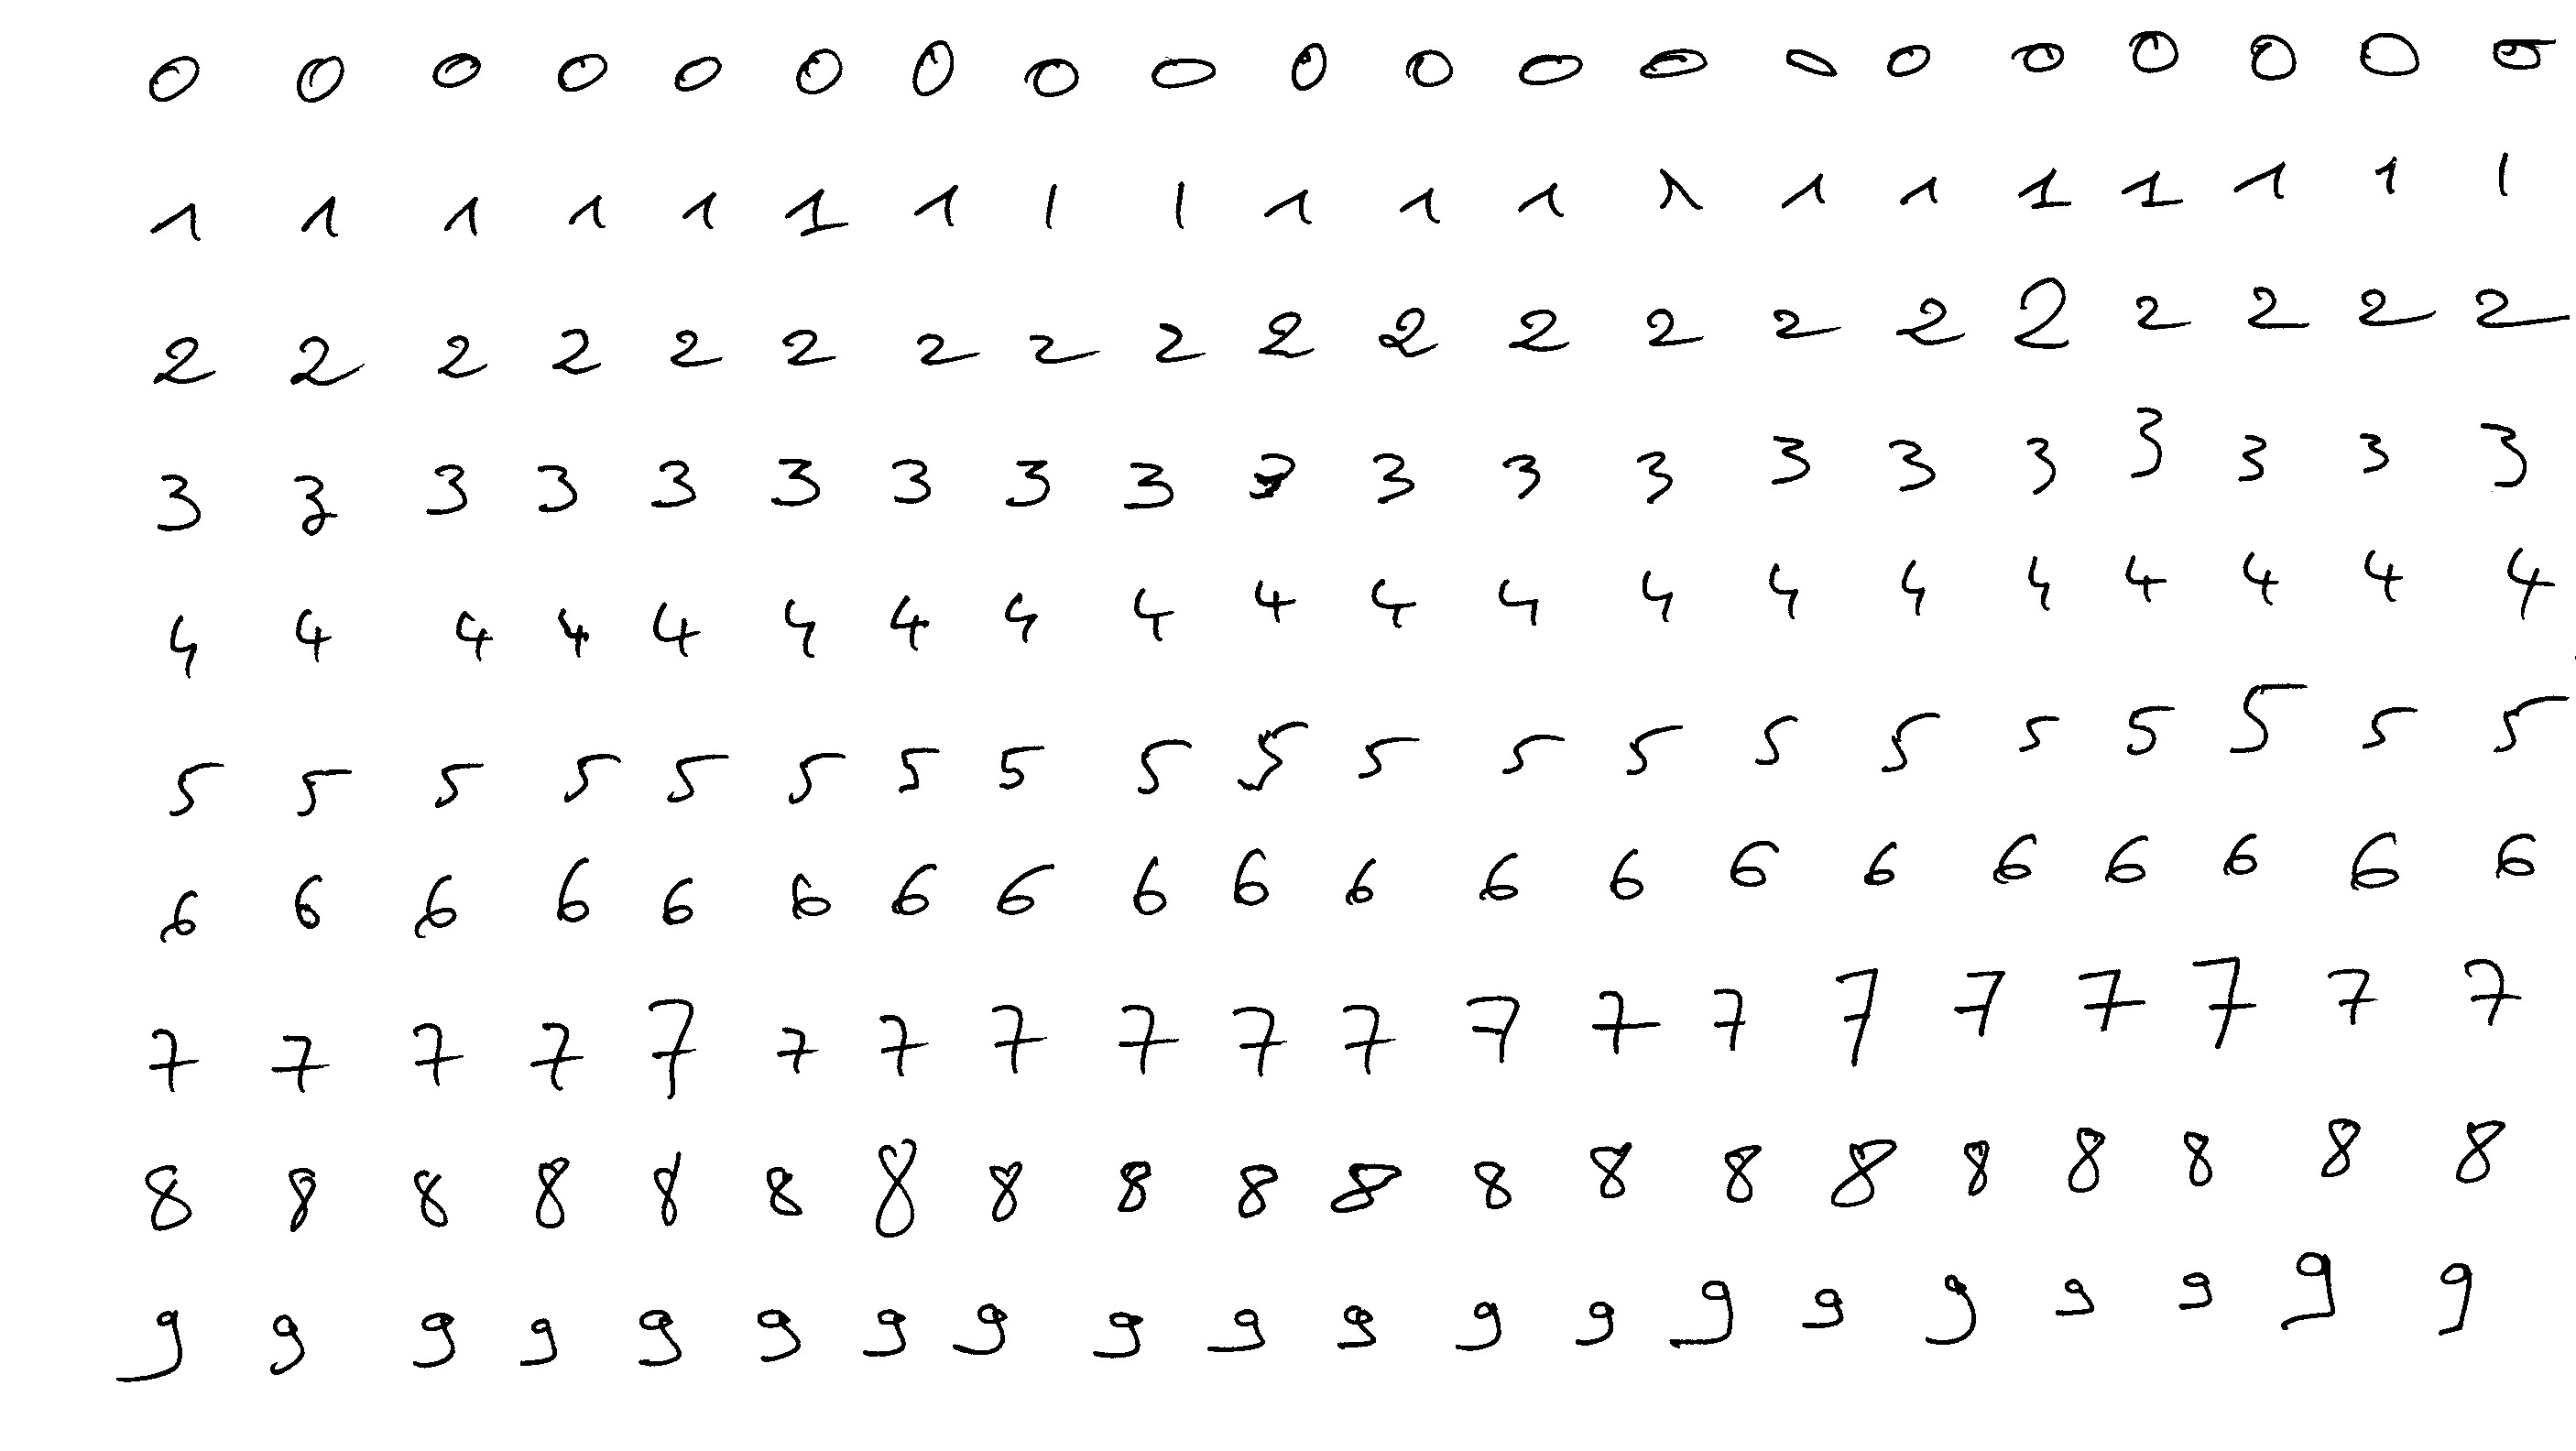
\includegraphics[scale=0.5]{app.jpg}
\caption{Base d'apprentissage du projet (200 chiffres)}
\end{figure}

\begin{figure}[!h]
\centering
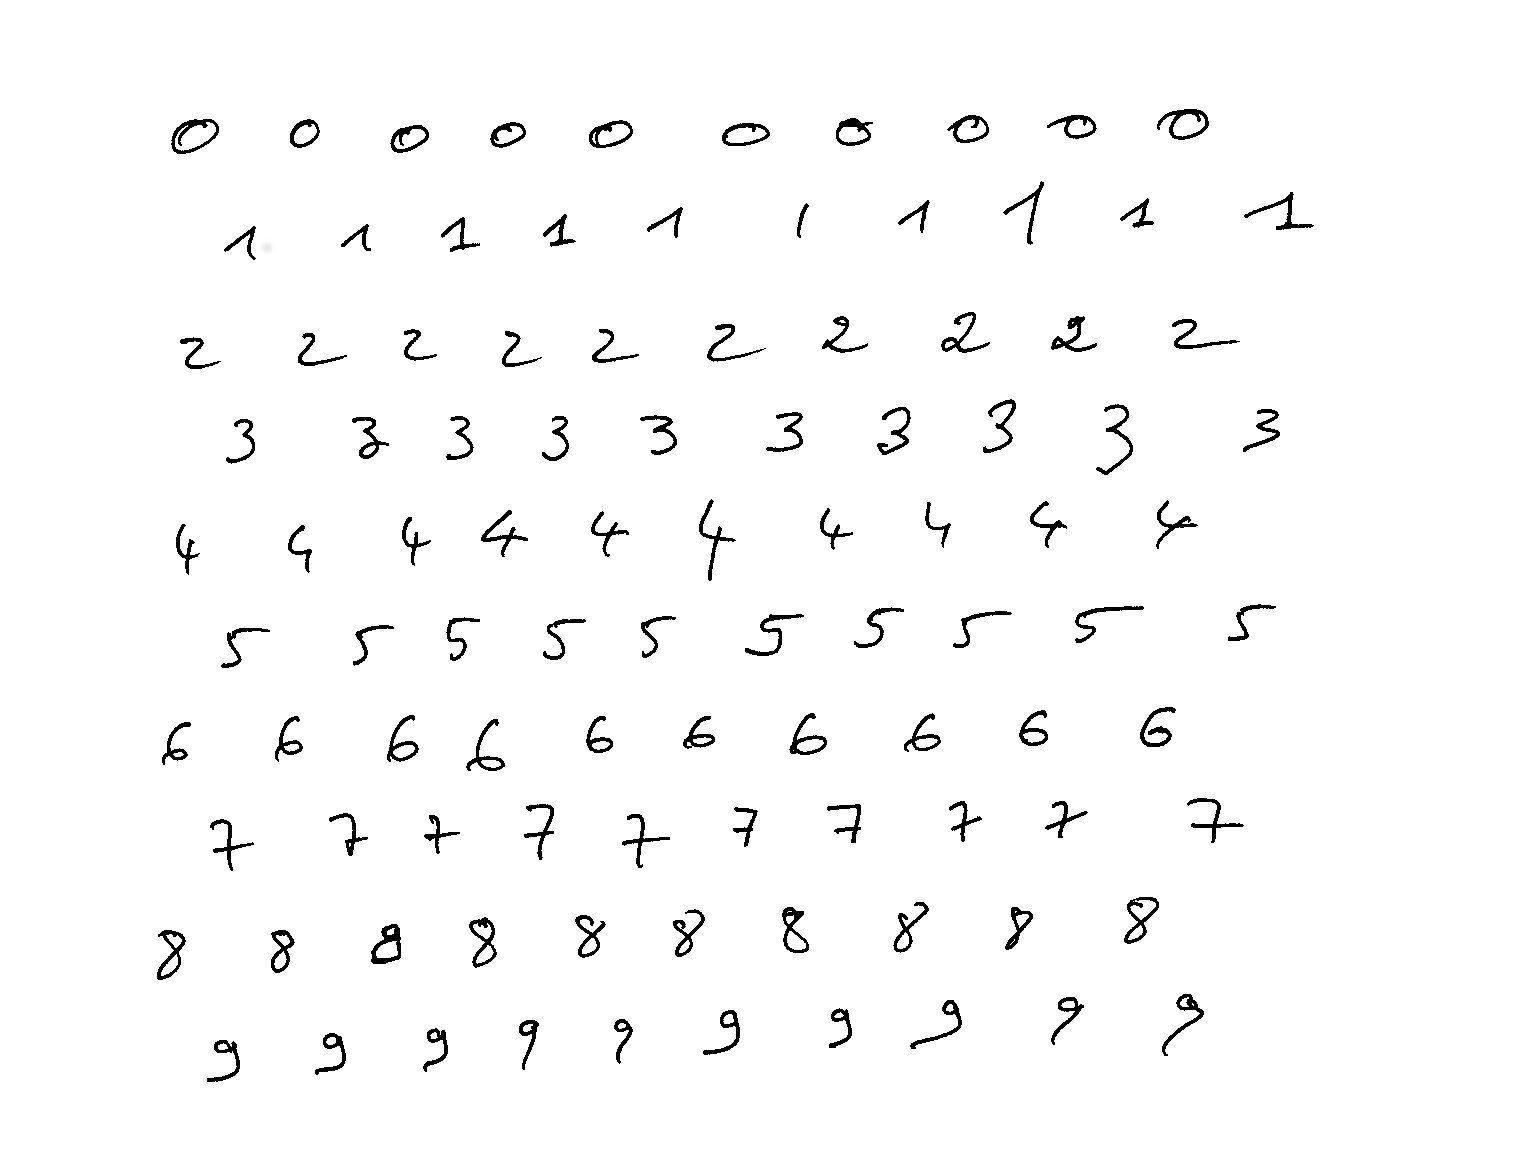
\includegraphics[scale=0.5]{test.jpg}
\caption{Base de test du projet (100 chiffres)}
\end{figure}


\chapter{Découpe des imagettes}
Comme nous le voyons sur les figures représentant les bases 
de chiffre qui nous sont données, les chiffres ne sont pas 
encore découpées. Pour procéder au découpage des imagettes, nous
avons utiliser les fonctions données par M. Chatelain. Celles-ci
ont été condensées en un fichier \texttt{crop\_image.m}. Celui-ci
contient une fonction MATLAB permettant de renvoyer un tableau 
d'images croppées.

\chapter{Apprentissage du modèle}
Pour réaliser notre projet, nous pouvions utiliser tout un panel
de caractéristiques adaptées à la reconnaissance de formes. Ces 
caractéristiques permettent d'obtenir des informations sur chaque
échantillon et ainsi de créer une \og carte d'identité \fg pour
chaque chiffres. Il sera ainsi plus facile de comparer la base
d'apprentissage aux échantillons de la base de test. \\
Les caractéristiques proposées par M. Chatelain dans l'énoncé du
projet sont au nombre de deux. La première consiste en l'élaboration
de profils pour chaque imagette. C'est la première méthode que
nous avons décidé d'implémenter. Suite à une petite étude que nous
avons fait, nous avons constaté que la méthode était optimal pour un
nombre de profils de 10. \\
La seconde méthode consiste en l'étude de densité de pixels au sein de 
l'imagette. Encore une fois, nous avons déterminé que les meilleurs
paramètres pour l'utilisation de cette méthode consiste à diviser 
l'imagette en 10 rangées pour 5 colonnes. \\
Après extraction complète du modèle, celui-ci se trouve dans une 
matrice qui sauvegarde pour chaque imagette toute les caractéristiques.
Cette matrice est enregistré sous la forme \texttt{modeleRDF.mat}.

\chapter{Classification}
Nous devons maintenant élaborer des classifieurs pour classer
les imagettes de la base de test dans différentes classes de chiffres.
Nous avons mis en place deux méthodes de classification. La première se 
base sur la distance euclidienne minimale du modèle par rapport à une
imagette de la base de test. La seconde consiste à réaliser la méthode des
$ k $ plus proches voisins. Nous nous sommes exclusivement concentrés sur les taux de réussite en TOP1.

\section{Reconnaissance avec distance euclidienne
minimale sur modèle moyen}

Cette méthode de classification consiste à comparer notre imagette de
test avec le modèle moyen pour chaque classe.
Avec cette méthode, nous obtenons la matrice de confusion suivante.

\begin{figure}[!h]
\centering
\begin{tabular}{|*{11}{c|}}
    \hline
     & 0 & 1 & 2 & 3 & 4 & 5 & 6 & 7 & 8 & 9 \\
    \hline
    0 & 1 & 0  & 0  & 0  & 0  & 0 & 0 & 0 & 0 & 0 \\
    \hline
    1 & 0 & 0.9 & 0.1 & 0  & 0 & 0 & 0 & 0 & 0 & 0 \\
    \hline
    2 & 0 & 0 & 0.9 & 0 & 0 & 0 & 0.1 & 0 & 0 & 0 \\
    \hline
    3 & 0 & 0 & 0 & 0.5 & 0 & 0 & 0 & 0 & 0 & 0.5 \\
    \hline
    4 & 0 & 0 & 0 & 0 & 0.9 & 0 & 0.1 & 0 & 0 & 0 \\
    \hline
    5 & 0 & 0 & 0 & 0 & 0 & 1 & 0 & 0 & 0 & 0 \\
    \hline
    6 & 0 & 0 & 0 & 0 & 0 & 0 & 1 & 0 & 0 & 0 \\
    \hline
    7 & 0 & 0 & 0 & 0.1 & 0 & 0 & 0 & 0.9 & 0 & 0 \\
    \hline
    8 & 0 & 0.2 & 0 & 0 & 0 & 0 & 0 & 0 & 0.8 & 0 \\
    \hline
    9 & 0 & 0 & 0 & 0 & 0 & 0 & 0 & 0.1 & 0.3 & 0.6 \\
    \hline
\end{tabular}
\caption{Matrice de confusion en TOP1 pour cette méthode}
\end{figure} 

Ceci nous donne 85\% de bons résultats avec ce classifieur.

Si nous choisissons en revanche de ne pas utiliser le modèle moyen
pour chaque classe mais, au contraire, d'utiliser la norme euclidienne
sur chaque élément du modèle, nous obtenons un résultat de 92\% en TOP1. Voici 
les résultats pour chaque classe.

\begin{figure}[h!]
\centering
\begin{tabular}{|*{10}{c|}}
    \hline
    0 & 1 & 2 & 3 & 4 & 5 & 6 & 7 & 8 & 9 \\
    \hline
    1 & 1 & 1 & 0.7 & 1 & 1 & 1 & 0.9 & 1 & 0.6  \\
    \hline
\end{tabular}
\caption{Résultat sans moyenner les classes}
\end{figure} 

Nous constatons que les chiffres soulevant le plus de problèmes sont 
le 9 et le 3. Il faudra donc trouver une méthode pour mieux les repérer.

\section{Décision par la méthode des k plus proches voisins}

Grâce au cours de Data-mining, nous savons écrire l'algorithme des k-ppvs.
Mais comment déterminer le nombre de plus proches voisins à sélectionner ?
Nous avons choisi, pour répondre à cette problématique, d'essayer 
avec plusieurs k différents. 

\begin{figure}[h!]
\centering
\begin{tabular}{|*{4}{c|}}
    \hline
    0.92 & 0.93 & 0.90 & 0.91 \\
    \hline
\end{tabular}
\caption{Bons résultats en TOP1 selon la valeur de k (k = 1, 2, 3, 4)}
\end{figure} 

Ceci nous amenant en toute logique à utiliser un k égal à 2.

\section{Méthode des k-ppvs avec d'autres distances}

Pour essayer d'améliorer nos résultats, nous avons voulu essayer
d'utiliser de nouvelles distances. Nous nous sommes donc intéressés
dans un premier temps à la distance de Manhattan. Celle-ci nous donne 
les résultats suivants.

\begin{figure}[h!]
\centering
\begin{tabular}{|*{10}{c|}}
    \hline
    0 & 1 & 2 & 3 & 4 & 5 & 6 & 7 & 8 & 9 \\
    \hline
    1 & 1 & 1 & 0.9 & 0.9 & 1 & 1 & 0.9 & 0.9 & 0.6  \\
    \hline
\end{tabular}
\caption{Résultat avec la distance de Manhattan}
\end{figure} 

Ceci donnant un résultat moyen de 92 \%, ce qui est insuffisant
comparé aux méthodes précédentes.

Nous avons ensuite essayé avec la distance de Minkowski de degré 3.
Celle-ci nous donne les résultats suivants.

\begin{figure}[h!]
\centering
\begin{tabular}{|*{10}{c|}}
    \hline
    0 & 1 & 2 & 3 & 4 & 5 & 6 & 7 & 8 & 9 \\
    \hline
    1 & 1 & 1 & 0.9 & 1 & 1 & 1 & 1 & 0.9 & 0.6  \\
    \hline
\end{tabular}
\caption{Résultat avec la distance de Minkowski}
\end{figure} 

Ceci donnant un résultat moyen de 94 \%, ce qui est déjà un meilleur
résultat. C'est donc très encourageant.

\section{Utilisation d'autres caractéristiques}

A cette étape du projet, nous avons choisi d'utiliser d'autres     
caractéristiques. En effet, les tests réalisés sur les classifieurs
ne montrait pas de grosses améliorations. \\
Nous nous sommes intéressés à la trace. Il s'agit en quelque sorte, 
de réaliser un profil sur un nombre de traits égal au nombre de pixel de
l'image. La figure suivante permet de visualiser les effets de notre
fonction \texttt{traceGD.m}.

\begin{figure}[h!]
\centering
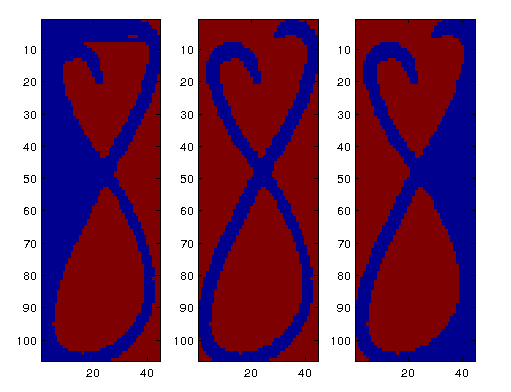
\includegraphics[scale=0.5]{trace.png}
\caption{Exemples de résultats de la fonction trace}
\end{figure}

Les résultats avec cette caractéristique sont les suivants :

\begin{figure}[h!]
\centering
\begin{tabular}{|*{2}{c|}}
    \hline
    kppv/trace Gauche & 0.88 \\
    \hline
    DEG/trace Gauche & 0.87 \\
    \hline
    kppv/trace Droite & 0.93 \\
    \hline
    DEG/trace Droite & 0.93 \\
    \hline
\end{tabular}
\caption{Taux de bons résultats avec la caractéristique trace}
\end{figure}

Nous avons aussi réalisé une méthode de classification par les kppvs
avec l'utilisation d'une trace Gauche-Droite qui donne des résultats 
peu intéressants mais qui reconnaît bien les 9. Il s'agirait donc de 
l'utiliser avec un classifieur plus efficace pour obtenir un très bon
taux de reconnaissance.

\section{Combinaison de classifieurs}

Nous allons donc essayer de combiner les classifieurs kppv/Minkowski3 avec la 
DEG/trace Droite et la DEG/trace Gauche-Droite. Nous choisirons les
paramètres optimaux dans le maximum de cas. \\
La combinaison de ces classifieurs commence par les classifieurs les plus
précis pour terminer avec le moins efficace mais qui discrimine mieux 
les 9 des 8. \\
Dans chaque cas, on vérifiera si le résultat obtenu est certain avec le classifieur utilisé.\\
S'il ne l'est pas, on passe au classifieur suivant pour essayer de déterminer avec exactitude la classe.

\section{Résultats finaux}

L'utilisation d'une combinaison de classifieurs nous a permis d'obtenir
de très bons résultats. En effet, nous avons réussi à obtenir un
taux de bonnes réponses de 98\%, voir le vecteur de résultat suivant.

\begin{figure}[h!]
\centering
\begin{tabular}{|*{10}{c|}}
    \hline
    0 & 1 & 2 & 3 & 4 & 5 & 6 & 7 & 8 & 9 \\
    \hline
    1 & 1 & 1 & 0.9 & 1 & 1 & 1 & 1 & 0.9 & 1  \\
    \hline
\end{tabular}
\caption{Résultat des classifieurs combinés}
\end{figure} 

Les confusions restantes sont obtenues sur un 3 et un 8 que notre
chaîne de reconnaissance de formes confond avec des 9. 


\chapter{Conclusion}
Nous venons de voir que la reconnaissance de formes est sensible 
aux parametres initiaux et aux caractéristiques utilisées. En combinant
des méthodes plutôt basiques et pas toujours efficaces globalement, 
on peut créer une très bon classifieur. \\
Ce fut un projet passionant et qui a révélé chez nous un certain 
enthousiasme pour la reconnaissance de formes. Nous avons pris un 
certain plaisir à réaliser ces algorithmes pour tenter d'obtenir
le meilleur résultat possible. Obtenir un résultat final de 98 \%
de bonnes réponses est pour nous une grande réussite.


\end{document}